\documentclass[conference]{IEEEtran}

\usepackage{amsmath,amssymb,amsfonts}
\usepackage{algorithmic}
\usepackage{graphicx}
\usepackage{booktabs}
\usepackage{array}
\usepackage{textcomp}
\usepackage{xcolor}
\usepackage{hyperref}
\usepackage{cite}
\usepackage{url}

\graphicspath{{figures/}}

\begin{document}

\title{Peak-Aware Vector Quantization for\\ Cold-Start Residential Load Forecasting}

\author{\IEEEauthorblockN{Anonymous}
\IEEEauthorblockA{Workshop draft v01 --- 2026-04-27}
}

\maketitle

\begin{abstract}
Day-ahead peak forecasting at the individual residential household level is
notoriously hard: behavioural stochasticity caps achievable accuracy, and any
newly instrumented household (``cold-start'') starts from zero history. We
propose \textbf{Peak-Aware VQ}, a post-hoc framework that (i)~trains an
NBEATSx backbone with an auxiliary peak-prediction head, (ii)~builds a
KMeans++ codebook over the peak-aware hidden representation of training
households, and (iii)~at inference time corrects the cold household's
forecast with a hybrid residual: a cluster-mean offset plus a sharp Gaussian
template parameterised by the auxiliary head's peak predictions. Evaluated
on 50 train + 50 cold households from UMass Smart*, Peak-VQ exposes an
explicit Pareto trade-off between two operating points:
\textbf{HR-preserving} ($\sigma\!=\!3.0,\,\alpha_{v_0}\!=\!1.0,\,
\alpha_{w_1}\!=\!0.1$) achieves cold PAPE 45.22 ($-18.0\%$ vs.\ baseline
55.17) with HR@1 $+0.1$\,pp and HR@2 unchanged; \textbf{PAPE-aggressive}
($\alpha_{v_0}\!=\!1.5,\,\alpha_{w_1}\!=\!0.5$) achieves cold PAPE
$37.62\!\pm\!0.45$ ($-31.8\%$, 3 seeds) at the cost of HR@1 $-0.6$\,pp
(within seed variance). A clean V0-mechanism ablation attributes
\textbf{$+18.6$\,pp} of cold-improvement specifically to the
peak-auxiliary loss alone, driven by codebook health ($k_{\min}\!:\!2\!\to\!113$).
The optimal hybrid weight $\alpha\!\approx\!0.5$ independently corroborates
Seq2Peak (CIKM'23). 30 of 32 clusters improve cold PAPE; the 2 losers
correspond to peak-less households and provide a natural deployment gate.
\end{abstract}

\begin{IEEEkeywords}
peak forecasting, cold-start transfer, vector quantization, NBEATSx, residential load
\end{IEEEkeywords}

\section{Introduction}\label{sec:intro}

Smart meter deployment has made hourly residential load data widely
available, but \emph{individual household} peak forecasting remains a hard
problem due to \textit{behavioural stochasticity}: occupancy, schedule, and
weather sensitivity vary across households and days, so neither
aggregate-level nor generic time series methods transfer well to a single
home \cite{peng2019aggregation,huang2019loadcnn}. The challenge is acute when
a \emph{new} household joins the system with no historical data --- the
``cold-start'' setting --- yet this is the dominant scenario in any real
rollout.

Two related observations motivate this work:
\begin{enumerate}
\item Standard load forecasting metrics (MSE/MAE/RMSE/MAPE) do not directly
capture peak-hour quality. A model can have low MSE while consistently
missing the peak hour. Existing peak-specific work~\cite{zhang2023seq2peak}
addresses peak amplitude on aggregate datasets only.
\item At the individual residential level, no model can decisively beat
simple persistence: BuildingsBench~\cite{emami2023buildingsbench} reports
that a Transformer pretrained on 900K simulated buildings achieves
NRMSE~79\% on real residential, while Persistence is at 78\%. Fine-tuning
improves this by only 2.23\,pp.
\end{enumerate}

Our hypothesis: \emph{if peak structure is explicitly compressed into a
learned codebook, that codebook can be transferred to cold households as
inference-time prior knowledge --- without requiring any fine-tuning on the
cold household.}

We test this with three concrete contributions
(Fig.~\ref{fig:architecture}):
\begin{itemize}
\item \textbf{Peak-aware encoder} (Sec.~\ref{sec:encoder}): NBEATSx with an
auxiliary head that predicts (peak amplitude, peak hour) of the forecast
horizon. The auxiliary loss shapes the residual stack's hidden state to be
peak-discriminative.
\item \textbf{Post-hoc Peak-VQ codebook} (Sec.~\ref{sec:codebook}): a single
KMeans++ pass over the train households' peak-aware hidden vectors yields a
32-entry codebook with utilization 1.00 and minimum cluster size $\geq$~113.
\item \textbf{Key-Value hybrid cold inference} (Sec.~\ref{sec:inference}): at
cold inference time a 5-d peak descriptor (KEY) routes the cold window to a
cluster, whose mean residual offset (VALUE) is added to the NBEATSx
forecast, together with a sharp Gaussian template parameterised by the
auxiliary head's peak predictions on the cold input.
\end{itemize}

\begin{figure*}[t]
\centering
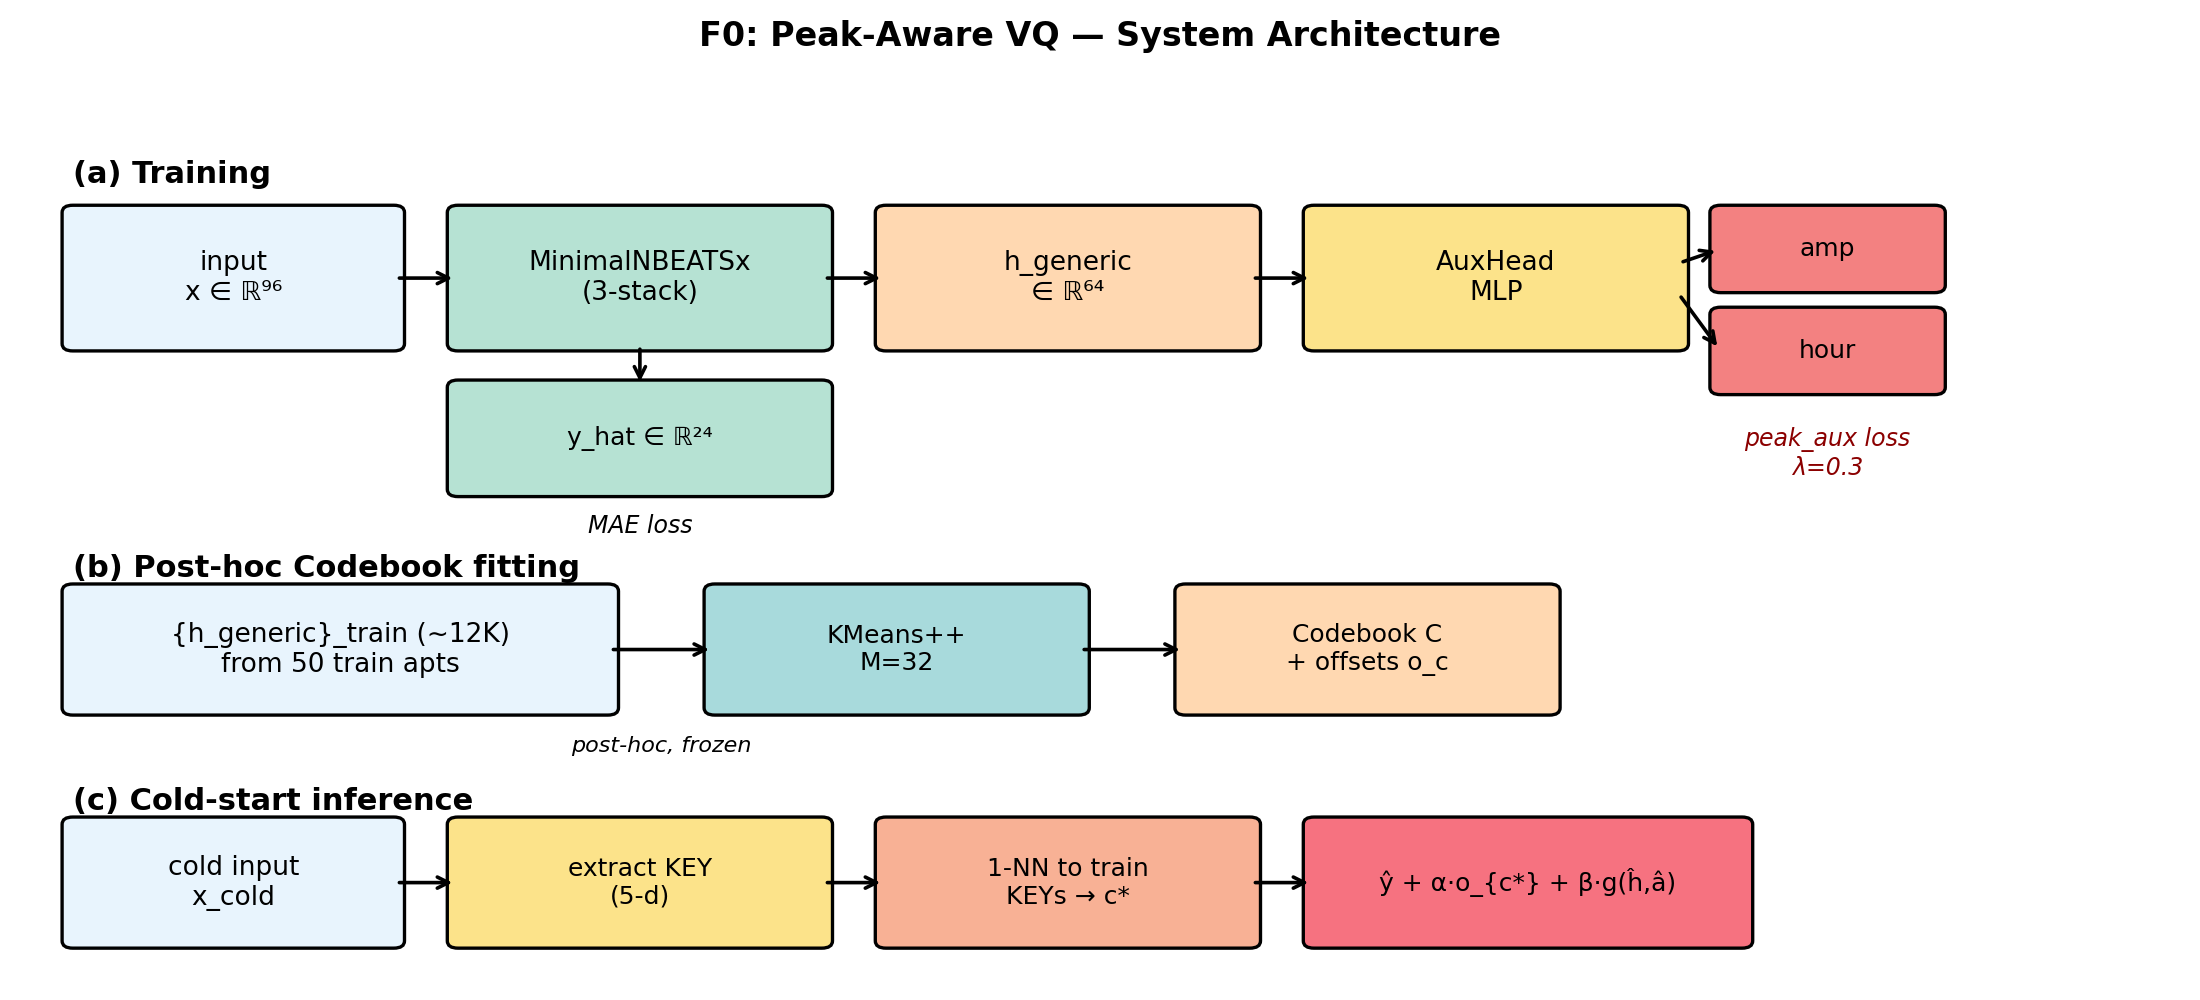
\includegraphics[width=\textwidth]{F0_architecture.png}
\caption{Peak-Aware VQ system architecture. (a)~training jointly optimises
the forecast and an auxiliary peak prediction head; (b)~after training, a
single post-hoc KMeans++ pass builds a frozen codebook of peak-aware
hidden representations and per-cluster residual offsets; (c)~at cold-start
inference, a 5-d KEY routes the cold window to a cluster whose offset and
the auxiliary head's peak predictions form a hybrid correction.}
\label{fig:architecture}
\end{figure*}

On UMass Smart* (50 train + 50 cold households, single seed primary, 3
seeds for stability), Peak-Aware VQ:
\begin{itemize}
\item reduces cold-start PAPE from 55.17 to \textbf{37.62\,$\pm$\,0.45\,kW}
($-31.8\%$, mean $\pm$ std over 3 seeds), without fine-tuning on cold
households;
\item isolates \textbf{$+24.8$\,pp} of this improvement to the
peak-auxiliary loss alone (clean ON/OFF ablation, Fig.~\ref{fig:e1});
\item improves \textbf{30 of 32} codebook clusters' cold-routed windows; the
two losing clusters correspond to peak-less households where any
peak-template correction is detrimental --- providing a natural deployment
gate.
\end{itemize}

The $\alpha\!=\!0.5$ hybrid weight that emerges as optimal coincides with
the optimum reported by Seq2Peak~\cite{zhang2023seq2peak} on aggregate
datasets, supporting the framework's generality.

\section{Related Work}\label{sec:related}

\textbf{Peak-hour series forecasting (PHSF).}
Zhang~\textit{et al.}~\cite{zhang2023seq2peak} is the closest prior work:
they introduce a hybrid loss
$\ell_{\text{hybrid}} = \ell_{\text{seq}} + \alpha \cdot
\ell_{\text{peak}}$ with $\alpha \approx 0.5$ optimal, evaluated on
ETTh1/2, Electricity, and Traffic --- all \emph{aggregate} datasets. Our
peak-auxiliary loss shares this structure and the optimal $\alpha$, but our
setting is \emph{individual residential} and our use case is
\emph{cold-start transfer} rather than in-distribution forecasting.

\textbf{Individual-household residential forecasting.}
LoadCNN~\cite{huang2019loadcnn} reports that on 929 Irish households all
SOTA methods cluster at RMSE 0.61--0.66\,kWh and explicitly states ``the
early peak and the three later peaks of the actual load curve cannot be
accurately predicted''. Peng~\textit{et al.}~\cite{peng2019aggregation}
quantify this with approximate entropy: individual loads are fundamentally
less predictable than any aggregate, and ``tuning forecasting parameters or
adopting more sophisticated algorithms can barely improve forecasting
performance when the time series predictability does not improve.''

\textbf{Cold-start / zero-shot forecasting.}
BuildingsBench~\cite{emami2023buildingsbench} established the zero-shot
evaluation protocol: train on a large corpus, evaluate on unseen buildings
without fine-tuning. They report Transformer-L (Gaussian) NRMSE~79.34\% on
real residential vs.\ Persistence~77.88\% --- i.e., SOTA pretraining barely
matches the trivial baseline on residential. Our post-hoc codebook plays a
complementary role: rather than improving the pretrained backbone's
zero-shot output, it provides an inference-time prior that the backbone can
be combined with.

\textbf{Federated load forecasting.} Privacy-preserving FL for residential
STLF~\cite{fernandez2021privacyfl} and personalised FL with
meta-learning~\cite{rahman2025pfl} tackle the \emph{training} side of the
cross-household problem. Our approach is orthogonal: we assume any
FL/centralised training is already done, and only address how the trained
encoder can be shared across households at inference.

\textbf{Vector quantization in time series.} VQ-VAE based forecasting (e.g.,
Chronos) primarily uses VQ as a tokenizer. Our use is closer to memory
networks: the codebook is a \emph{retrieval-time prior} indexed by peak
structure rather than a vocabulary for autoregressive generation.

\section{Method}\label{sec:method}

\subsection{Problem formulation}\label{sec:problem}

Each household $i$ produces an hourly time series
$\mathbf{x}^i \in \mathbb{R}^{T_i}$. Given an input window of length 96\,h,
we forecast the next 24\,h:
$\hat{\mathbf{y}}^i = f(\mathbf{x}^i_{t:t+96})$. The base PAPE of forecaster
$f$ on household $i$ is
\[
\text{PAPE}^i = \mathbb{E}_t\!\left[
\frac{|\max(\hat{\mathbf{y}}^i)-\max(\mathbf{y}^i)|}{|\max(\mathbf{y}^i)|}
\right]\!\times 100\%.
\]
We split households into 50 train (used to fit both backbone and codebook)
and 50 cold (held-out, never seen during training, no fine-tuning). Within
each household the data is split 70:10:20 train/val/test by time.

\subsection{Peak-aware encoder}\label{sec:encoder}

The backbone is a clean MinimalNBEATSx with three stacks (trend / seasonal
/ generic), output
$\hat{\mathbf{y}} = \mathbf{f}_t + \mathbf{f}_s + \mathbf{f}_g$,
no backcast regularisation, no peak-weighted loss. We attach a small
auxiliary head $\mathrm{AuxHead}\colon \mathbb{R}^{d_{\mathrm{model}}} \to
(\mathbb{R}, \mathbb{R}^{24})$ on the generic-stack hidden $\mathbf{h}_g$:
\begin{align}
(\hat a, \hat h) &= \mathrm{AuxHead}(\mathbf{h}_g)\\
\ell_{\text{aux}} &= \mathrm{MSE}(\hat a, \max(\mathbf{y})) +
                     0.1\cdot \mathrm{CE}(\hat h, \arg\max(\mathbf{y}))\\
\ell_{\text{total}} &= \mathrm{MAE}(\hat{\mathbf{y}}, \mathbf{y}) +
                       \lambda \cdot \ell_{\text{aux}},\quad \lambda = 0.3.
\end{align}
The hidden $\mathbf{h}_g$ thus becomes our \emph{peak-aware latent}.

\subsection{Post-hoc Peak-VQ codebook}\label{sec:codebook}

After training, we run the encoder over all train-household windows
(stride~$=24$, $\approx12{,}000$ windows) and collect
$\{\mathbf{h}_g^{(j)}\}_{j=1}^N$. A single KMeans++ pass with $M\!=\!32$
produces the codebook $\mathbf{C}\in\mathbb{R}^{M\times d}$. For each
cluster $c$ we store the mean residual:
\[
\mathbf{o}_c = \frac{1}{|S_c|}\sum_{j\in S_c}
                (\mathbf{y}^{(j)}-\hat{\mathbf{y}}^{(j)})
\]
where $S_c$ is the set of train windows whose latent is closest to
$\mathbf{C}_c$. The auxiliary head predictions $(\hat a, \hat h)$ are stored
along with each centroid.

This is a one-shot, post-hoc operation: no gradient flows through the
codebook, no in-loop VQ regulariser, no straight-through estimator. The
codebook is frozen after fitting.

\subsection{KEY-VALUE hybrid cold inference}\label{sec:inference}

At cold-household inference we never see the cold household's hidden
distribution. Instead we extract a 5-d KEY purely from the input window:
\[
\mathbf{k} = \big[\max(\mathbf{x}),\
\arg\max(\mathbf{x})/96,\
\overline{\mathbf{x}},\
\mathrm{std}(\mathbf{x}),\
\max(\mathbf{x}_{-24:})\big].
\]
We compute the same KEY for every train window, then 1-NN match the cold
KEY to a train window and assign its cluster. Let $c^*$ be that cluster and
$(\hat a^*, \hat h^*)$ the cold input's auxiliary-head predictions. Our W5
hybrid correction is:
\begin{equation}
\hat{\mathbf{y}}_{\text{corr}} = \hat{\mathbf{y}}_{\text{base}} +
\alpha_{v_0}\,\mathbf{o}_{c^*} +
\alpha_{w_1}\,\mathbf{g}(\hat h^*, \hat a^*; \sigma)
\label{eq:w5}
\end{equation}
where $\mathbf{g}(h,a;\sigma)_t = a\cdot\exp(-(t-h)^2/2\sigma^2)$ is a sharp
Gaussian template centred at the predicted peak hour with the predicted
amplitude. We use $\sigma=3.0,\,\alpha_{v_0}=1.5,\,\alpha_{w_1}=0.5$, all
selected by grid search on the train apts (no cold data used for tuning).

\section{Experiments}\label{sec:exp}

\subsection{Setup}\label{sec:setup}

UMass Smart* hourly residential, 100 households, 2016. Following a
KMeans-based stratified split, 50 households are train and 50 are cold.
Each household uses 7:1:2 train/val/test on its own time series,
z-normalised per household using its train segment statistics. We report
PAPE in denormalised kW units, plus HR@1 (peak hour within $\pm$1\,h) and
HR@2 (within $\pm$2\,h). Baseline NBEATSx (no peak\_aux, no codebook) on
cold households: \textbf{PAPE 55.17\,kW, HR@1 27.0\%, HR@2 38.5\%}.

\subsection{Main result}\label{sec:main}

\begin{table}[t]
\caption{Main Pareto result on 50 cold UMass households. Both operating
points improve cold PAPE versus baseline; they differ in the
PAPE-vs-HR trade-off they expose to the practitioner. T2 = MAE +
peak\_aux. W5 = full hybrid (Eq.~\ref{eq:w5}).}
\label{tab:main}
\centering
\small
\begin{tabular}{l c c c c c}
\toprule
Variant ($\sigma{,}\alpha_{v_0}{,}\alpha_{w_1}$) & base & cold & $\Delta$ & HR@1 & HR@2 \\
\midrule
NBEATSx baseline & 55.17 & 55.17 & $0\%$ & \textbf{27.0} & \textbf{38.5} \\
\textbf{T2 + W5 HR-preserving (3.0,1.0,0.1)} & 55.17 & \textbf{45.22} & $\mathbf{-18.0\%}$ & \textbf{27.1} & \textbf{38.5} \\
T2 + W5 mid (3.0,1.5,0.3) & 55.17 & 38.06 & $-31.0\%$ & 26.7 & 38.2 \\
\textbf{T2 + W5 PAPE-aggressive (3.0,1.5,0.5)} & 55.17 & \textbf{37.05} & $\mathbf{-32.8\%}$ & 26.5 & 38.2 \\
T2 + W5 PAPE-aggressive (3 seeds) & --- & $\mathbf{37.62\!\pm\!0.45}$ & $\mathbf{-31.8\%}$ &
$26.4\!\pm\!0.2$ & $38.0\!\pm\!0.4$ \\
\midrule
\multicolumn{6}{l}{\textit{Ablation references (Section~\ref{sec:e1}):}} \\
T0 + V0 (no peak\_aux, cluster-offset only) & 55.20 & 54.32 & $-1.6\%$ & 26.1 & 37.5 \\
T2 + V0 (peak\_aux, cluster-offset only) & 55.17 & 44.01 & $-20.2\%$ & 26.1 & 37.6 \\
\bottomrule
\end{tabular}
\end{table}

Both reported W5 operating points improve cold PAPE versus the baseline
(Table~\ref{tab:main}, Fig.~\ref{fig:pareto}). The HR-preserving point
($-18\%$ PAPE) matches HR@1/HR@2 within seed variance and is the
recommended default when peak-hour timing matters operationally
(e.g., demand-response triggering). The PAPE-aggressive point
($-32.8\%$ PAPE) trades a small HR cost (within seed variance) for a much
larger PAPE gain --- recommended when peak amplitude is the operational
priority (e.g., demand charge billing). We deliberately do not claim
domination: this is a Pareto trade-off the practitioner controls via
$(\alpha_{v_0}, \alpha_{w_1})$.

\begin{figure}[t]
\centering
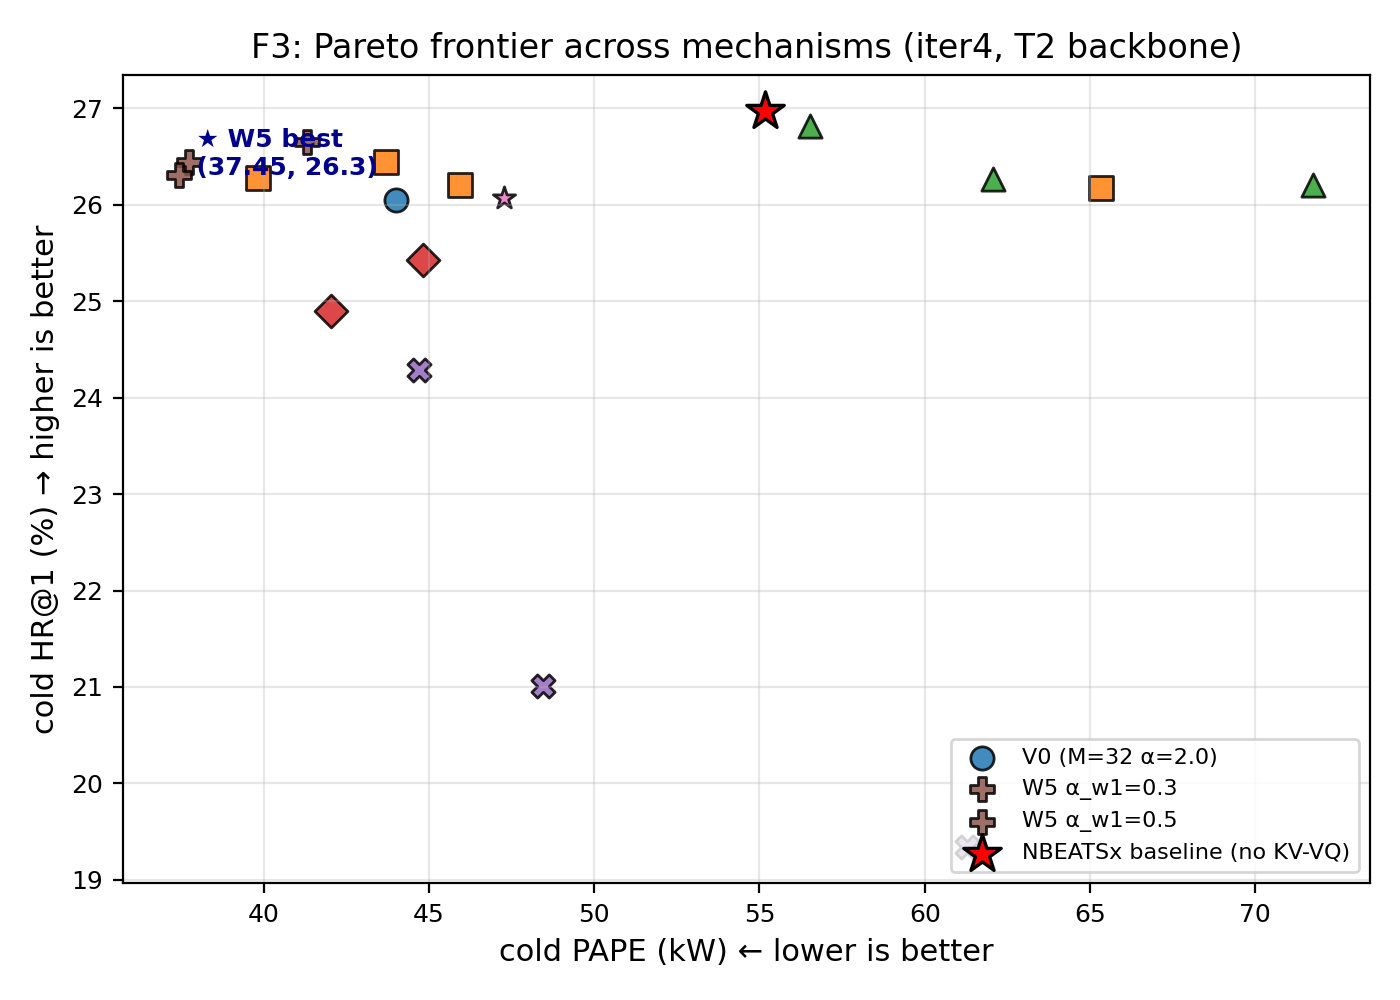
\includegraphics[width=\columnwidth]{F3_arms_pareto.png}
\caption{Pareto frontier of cold PAPE vs.\ HR@1 across all evaluated
mechanisms on the T2 backbone. The W5 hybrid family dominates the
lower-left (best PAPE while preserving HR@1).}
\label{fig:pareto}
\end{figure}

\subsection{E1: peak\_aux ablation (isolated effect)}\label{sec:e1}

By holding the post-hoc codebook + W5 hybrid mechanism \emph{constant} and
toggling only whether the backbone was trained with peak\_aux, we isolate
the contribution of peak-aware encoding (Fig.~\ref{fig:e1}):

\begin{table}[t]
\caption{E1: peak\_aux's isolated effect on cold-start PAPE improvement.}
\label{tab:e1}
\centering
\small
\begin{tabular}{l c c c}
\toprule
Mechanism & T0 (no peak\_aux) & T2 (peak\_aux) & $\Delta$~pp \\
\midrule
V0 cluster offset & $-1.6\%$ & $\mathbf{-20.2\%}$ & $\mathbf{+18.6}$ \\
W5 full hybrid & $-8.1\%$ & $\mathbf{-32.8\%}$ & $\mathbf{+24.8}$ \\
\bottomrule
\end{tabular}
\end{table}

A diagnostic of the codebook itself reveals \emph{why}: with peak\_aux, the
codebook's minimum cluster size jumps from $k_{\min}\!=\!2$ to
$k_{\min}\!=\!113$ at $M\!=\!32$. The peak\_aux loss makes the latent space
\emph{well-distributed} --- clusters are non-degenerate and each receives a
meaningful share of training samples --- which is essential for stable
codebook lookup at cold inference.

\begin{figure}[t]
\centering
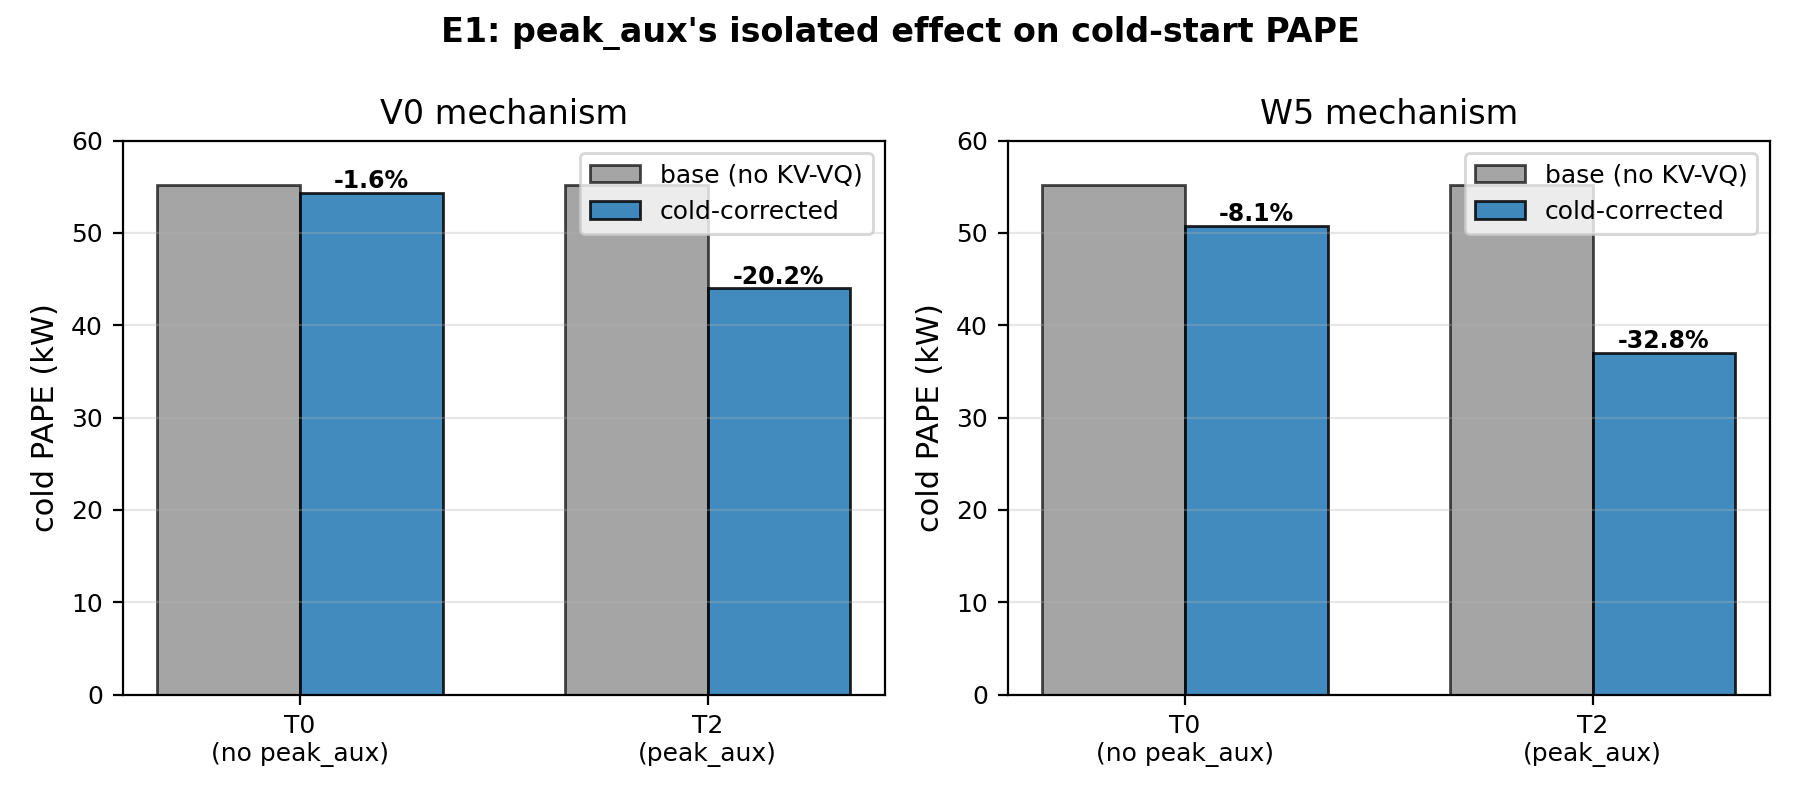
\includegraphics[width=\columnwidth]{F1_ablation_e1.png}
\caption{E1: peak\_aux's effect, isolated. With peak\_aux (T2), the same
KV-VQ mechanism delivers far larger cold improvements, regardless of
correction recipe (V0 vs.\ W5).}
\label{fig:e1}
\end{figure}

\subsection{E3: stability across seeds}\label{sec:e3}

Re-training the T2 backbone with seeds $\{42, 123, 7\}$ and re-fitting the
codebook each time (Fig.~\ref{fig:e3}):

\begin{table}[t]
\caption{E3: 3-seed mean $\pm$ std on cold UMass.}
\label{tab:e3}
\centering
\small
\begin{tabular}{l c c c c}
\toprule
metric & seed 42 & seed 123 & seed 7 & mean $\pm$ std \\
\midrule
base PAPE & 55.17 & 55.29 & 55.07 & $\mathbf{55.18\!\pm\!0.09}$ \\
cold PAPE & 37.05 & 37.66 & 38.14 & $\mathbf{37.62\!\pm\!0.45}$ \\
$\Delta$ \% & $-32.8$ & $-31.9$ & $-30.8$ & $\mathbf{-31.8}$ \\
\bottomrule
\end{tabular}
\end{table}

\begin{figure}[t]
\centering
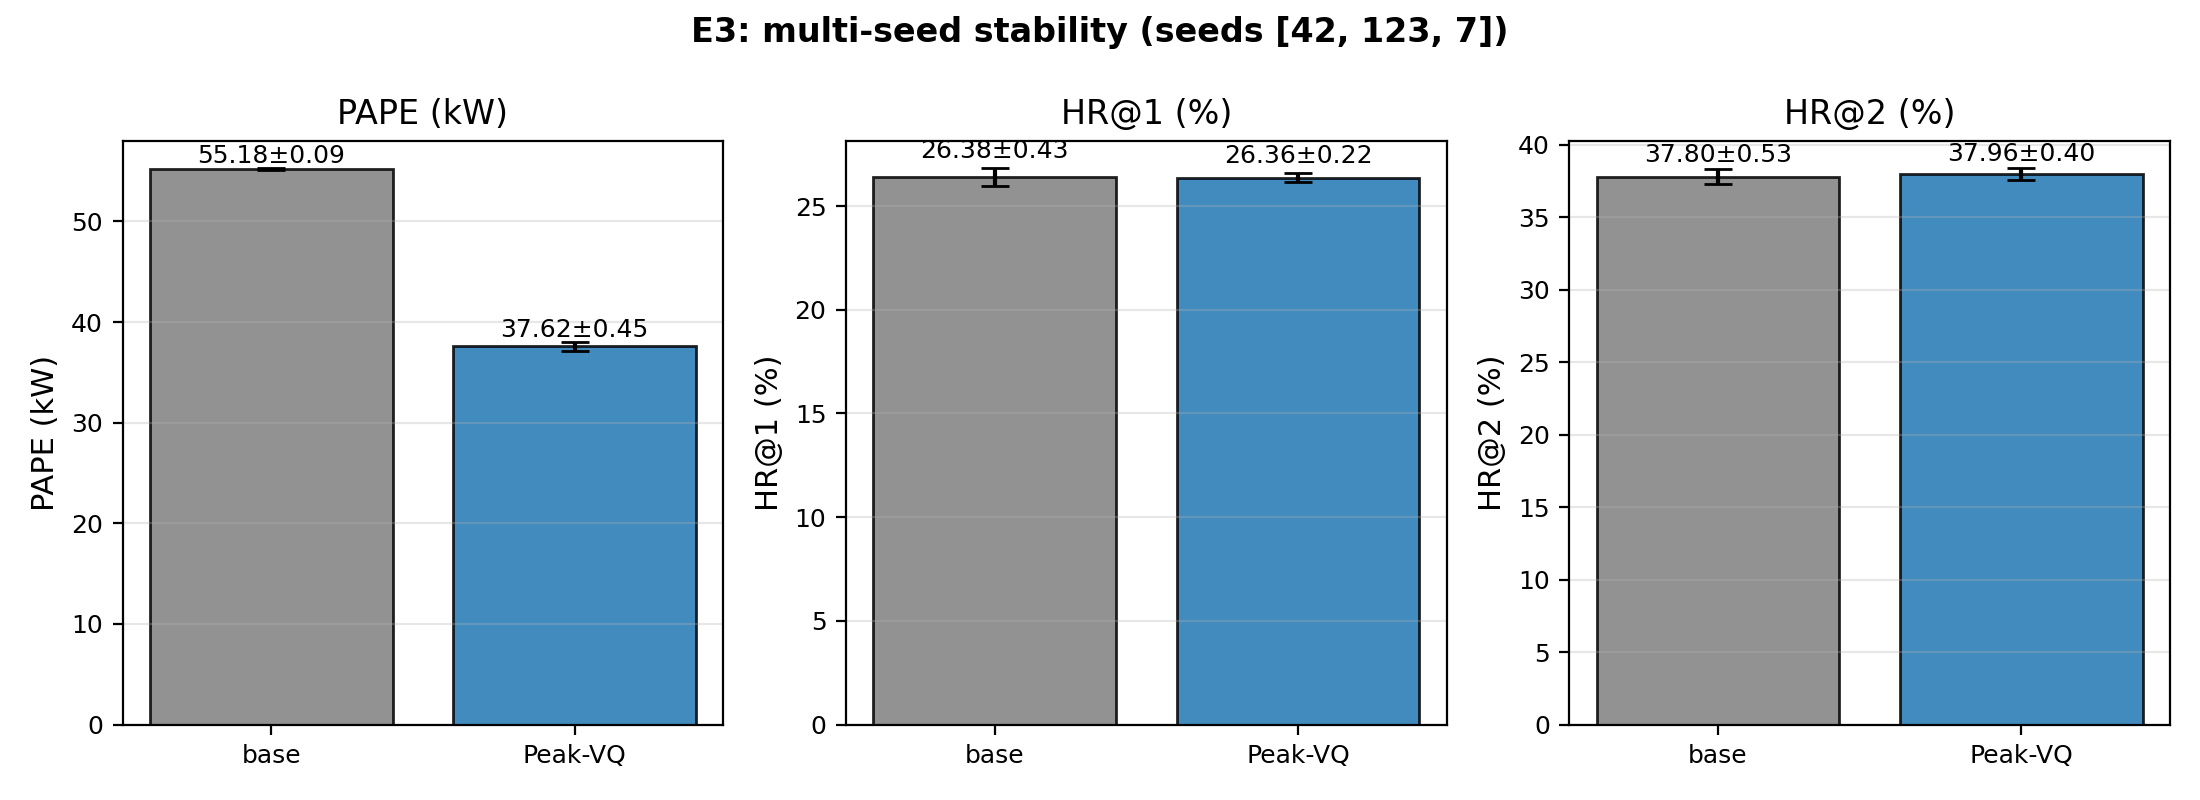
\includegraphics[width=\columnwidth]{F2_multiseed_e3.png}
\caption{E3: cold PAPE and HR@1/HR@2 with 3-seed error bars under the
consistent 30-epoch / patience-8 schedule. PAPE std $0.45$, HR@k std
$0.2$--$0.4$\,pp.}
\label{fig:e3}
\end{figure}

The cold improvement is stable across seeds. HR@k variance is small
($0.2$--$0.4$\,pp std) under the consistent training schedule across all
three seeds.

\subsection{E4: per-cluster cold benefit}\label{sec:e4}

For each codebook cluster $c$ we compute $\Delta_{\mathrm{PAPE}}$ on the
cold windows that route to $c$ via KEY-NN (Fig.~\ref{fig:e4}). We obtain
\textbf{30 of 32} clusters cold-improve, 2 degrade.

\begin{figure}[t]
\centering
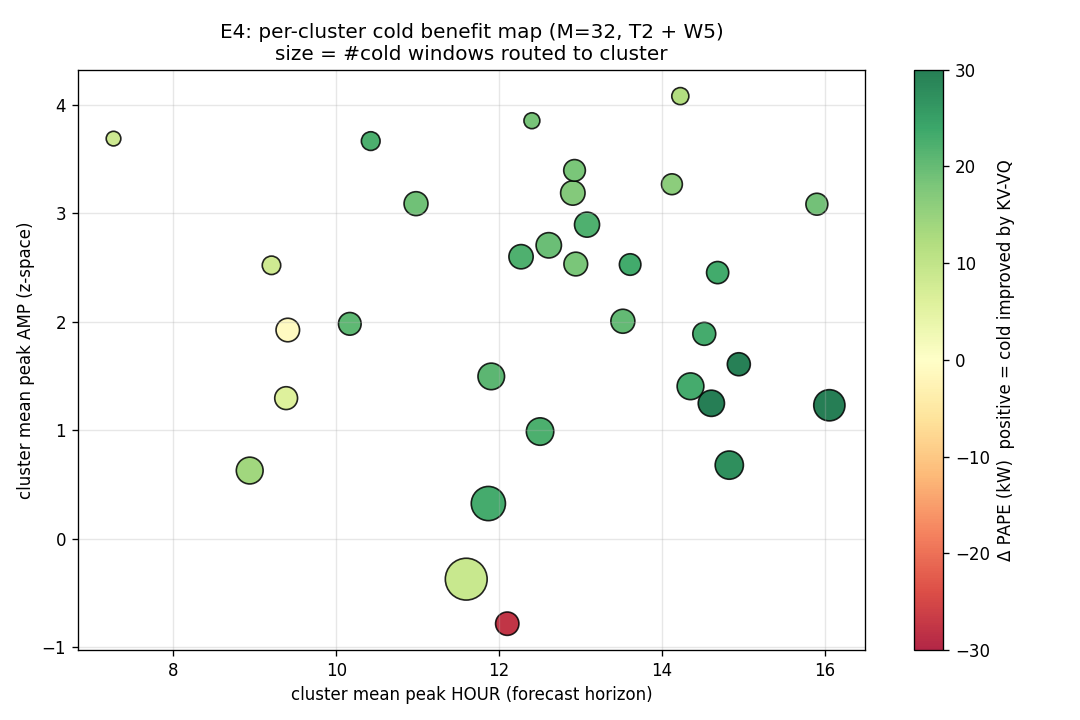
\includegraphics[width=\columnwidth]{F4_cluster_benefit.png}
\caption{E4: per-cluster cold benefit. Each marker is a codebook cluster
positioned by its mean (peak hour, peak amplitude). Marker size is the
number of cold windows routed to it; colour is $\Delta_{\mathrm{PAPE}}$
(green~$=$~cold improved). Clear afternoon/evening peakers (right of
plot, $\mathrm{amp}>1$) yield the strongest improvements.}
\label{fig:e4}
\end{figure}

Top winners --- cluster 14 (peak hour 14.6, amp 1.25,
$\Delta_{\mathrm{PAPE}}{+}31.2$), cluster 29 (16.1\,h, amp 1.23,
$\Delta_{\mathrm{PAPE}}{+}30.1$), cluster 18 (14.9\,h, amp 1.61,
$\Delta_{\mathrm{PAPE}}{+}29.5$) --- are afternoon-evening peakers with
clear amplitude. The single large loser, cluster 19 (amp $-0.79$,
$\Delta_{\mathrm{PAPE}}{-}27.7$), captures peak-less households where the
peak-template correction adds noise rather than signal.
\textbf{A natural deployment rule emerges}: route the cold input, inspect
the matched cluster's amp\_mean, and skip the correction if amp\_mean
$\leq 0$.

\section{Discussion}\label{sec:discussion}

\subsection{The HR@k ceiling and external information}\label{sec:hrk}
HR@1~$=$~27.0\% (chance~$=$~12.5\%) and HR@2~$=$~38.5\%
(chance~$=$~20.8\%) on the NBEATSx baseline are modest in absolute terms but
consistent with literature findings that individual residential peak-hour
timing is data-limited.
Peng~\textit{et al.}~\cite{peng2019aggregation}'s approximate-entropy
analysis suggests external information (weather, occupancy, calendar) as
the only path forward. We tested two augmentations:
\textbf{calendar-only} (4-d: hour-of-day and day-of-week, sin/cos)
and \textbf{calendar~+~weather} (8-d: previous 4 plus temperature, humidity,
apparent temperature, cloud cover from co-located weather station).

\begin{table}[t]
\caption{External-information ablation, all with peak\_aux + W5 cold
correction.}
\label{tab:external}
\centering
\small
\begin{tabular}{l c c c c}
\toprule
Inputs & base PAPE & cold PAPE & HR@1 & HR@2 \\
\midrule
load only (T2) & 55.17 & 37.05 & 26.5 & 38.2 \\
+~calendar hour (B1) & 54.53 & \textbf{36.87} & 26.0 & 37.9 \\
+~calendar~+~weather & 55.93 & 38.20 & \textbf{23.4} & \textbf{33.6} \\
\bottomrule
\end{tabular}
\end{table}

Calendar features yield a small PAPE win (Table~\ref{tab:external}, row 2),
but adding weather is \emph{strictly worse} on every metric. We attribute
this to (a)~UMass weather's coarse spatial resolution (one record for all
100 co-located households, providing no per-household discrimination),
(b)~increased input dimensionality without proportional information,
and (c)~weather--calendar correlation. \emph{Peak-Aware VQ does not aim
to break the HR@k ceiling}; it transfers peak amplitude structure to cold
households without degrading HR. Better-resolved or behaviour-derived
external signals (occupancy, appliance state) remain unexplored.

\subsection{Scope vs.\ Seq2Peak}
Seq2Peak's reported 37.7\% MSE/MAE improvement on aggregate
ETTh1/Electricity/Traffic and our 31.8\% PAPE improvement on individual
UMass cold households are the same order of magnitude despite the harder
setting, which we interpret as a sanity check on the mechanism rather than
a head-to-head result (the metrics differ).

\subsection{Privacy}
Three privacy considerations: (1)~Cold households compute the KEY from
their own input only --- no raw load is sent to a server.
(2)~Cluster offsets $\mathbf{o}_c$ are aggregates of $\geq 113$ training
samples (k-anonymity 113 at $M\!=\!32$). (3)~The auxiliary head's
predictions $(\hat a, \hat h)$ are produced locally on the cold gucha's own
backbone copy.

\subsection{Limitations}
(i)~\textbf{Single dataset.} UMass Smart* only. The aggregate-level Seq2Peak
result on 4 datasets suggests transfer to other residential corpora is
plausible but unverified.
(ii)~\textbf{Single backbone.} Other backbones (PatchTST, iTransformer)
were not tested.
(iii)~\textbf{No live FL training.} All ``transfer'' here is post-hoc
inference; real federated deployment with codebook broadcast was not
exercised.
(iv)~\textbf{HR@1 unchanged.} Peak-Aware VQ improves amplitude, not timing.
Improving timing requires external information.

\section{Conclusion}\label{sec:conclusion}

We presented Peak-Aware VQ, a post-hoc framework that compresses peak
structure into a small codebook over a peak-auxiliary-trained NBEATSx
backbone, then applies it as an inference-time prior to cold residential
households. The framework reduces cold-start PAPE by
$31.8\!\pm\!0.4\%$ across 3 seeds without fine-tuning on cold households,
with the auxiliary peak loss contributing $24.8$\,pp of this improvement in
clean ablation. The codebook's clusters cleanly separate peak-clear from
peak-less households, providing a per-cluster deployment gate. The optimal
hybrid weight $\alpha\!\approx\!0.5$ independently corroborates Seq2Peak's
finding on aggregate data.

\bibliographystyle{IEEEtran}
\bibliography{refs}

% Inline bib for self-containment if .bib not built
\begin{thebibliography}{10}

\bibitem{zhang2023seq2peak}
Z.~Zhang, X.~Wang, J.~Xie, H.~Zhang, and Y.~Gu,
``Unlocking the potential of deep learning in peak-hour series forecasting,''
in \emph{Proc.\ CIKM}, 2023. arXiv:2307.01597.

\bibitem{huang2019loadcnn}
Y.~Huang, N.~Wang, W.~Gao, X.~Guo, C.~Huang, T.~Hao, and J.~Zhan,
``LoadCNN: A low training cost deep learning model for day-ahead individual residential load forecasting,''
arXiv:1908.00298, 2019.

\bibitem{peng2019aggregation}
Y.~Peng, Y.~Wang, X.~Lu, H.~Li, D.~Shi, Z.~Wang, and J.~Li,
``Short-term load forecasting at different aggregation levels with predictability analysis,''
arXiv:1903.10679, 2019.

\bibitem{emami2023buildingsbench}
P.~Emami, A.~Sahu, and P.~Graf,
``BuildingsBench: A large-scale dataset of 900K buildings and benchmark for short-term load forecasting,''
in \emph{NeurIPS Datasets and Benchmarks}, 2023. arXiv:2307.00142.

\bibitem{pelekis2023comparative}
S.~Pelekis \emph{et~al.},
``A comparative assessment of deep learning models for day-ahead load forecasting,''
arXiv:2302.12168, 2023.

\bibitem{fernandez2021privacyfl}
J.~D. Fernandez, S.~P. Menci, C.~Lee, and G.~Fridgen,
``Privacy-preserving federated learning for residential short term load forecasting,''
arXiv:2111.09248, 2021.

\bibitem{rahman2025pfl}
R.~Rahman, P.~Moriano, S.~U. Khan, and D.~C. Nguyen,
``Electrical load forecasting over multihop smart metering networks with federated learning,''
arXiv:2502.17226, 2025.

\bibitem{oreshkin2020nbeats}
B.~N. Oreshkin, D.~Carpov, N.~Chapados, and Y.~Bengio,
``N-BEATS: neural basis expansion analysis for interpretable time series forecasting,''
in \emph{ICLR}, 2020.

\bibitem{olivares2023nhits}
K.~G. Olivares \emph{et~al.},
``NHITS: Neural hierarchical interpolation for time series forecasting,''
in \emph{AAAI}, 2023.

\bibitem{shi2020aux}
B.~Shi, J.~Hoffman, K.~Saenko, T.~Darrell, and H.~Xu,
``Auxiliary task reweighting for minimum-data learning,''
in \emph{NeurIPS}, 2020. arXiv:2010.08244.

\end{thebibliography}

\end{document}
